\chapter{Projetando um Ambiente Analítico}
\label{metodologia}
\section{Identificação de Dados}
\label{coleta}

A construção de um ambiente analítico voltado à mensuração de risco de ações exige, antes de qualquer modelagem, a definição precisa de quais dados serão observados, de onde eles serão obtidos e em que janela temporal a observação ocorrerá. Esta seção descreve, em nível conceitual, essas três decisões. Os detalhes operacionais da extração são apresentados no capítulo \ref{implementacao}.

\subsection{Universo de ativos analisados}

O universo de análise é composto pelas ações listadas nas duas principais bolsas norte-americanas: a NYSE e NASDAQ. A opção por esse recorte geográfico apoia-se em três fatores. Primeiro, o mercado acionário dos Estados Unidos é o que apresenta maior liquidez do mundo, oferecendo séries históricas longas, contínuas e com elevada qualidade de informação. Segundo, a cobertura setorial é abrangente, contemplando desde setores tradicionais (\textit{Industrials, Financial Services, Energy}) até setores intensivos em tecnologia (\textit{Technology, Communication Services}), o que viabiliza análises comparativas entre faixas de risco e perfis fundamentalmente distintos. Terceiro, a existência de um \textit{benchmark} amplamente aceito para esses dados, o índice S\&P~500, permite calibrar o risco sistemático dos ativos contra uma referência única e padronizada, conforme detalhado na Seção~\ref{sec:modelagem-risco}.

A listagem dos \textit{tickers}, que são códigos de identificação alfanuméricos usados na bolsa de valores para representar ativos negociados, como NVDA, referente à NVIDIA na NASDAQ, e os dados de mercado e fundamentos são obtidos a partir de um provedor público de dados financeiros, que agrega informações das bolsas norte-americanas e disponibiliza acesso programático tanto a séries históricas de cotação quanto a um conjunto de atributos descritivos por ativo. A base coletada abrange o universo completo de instrumentos negociados na NYSE e na NASDAQ, incluindo ações ordinárias, classes especiais, séries de ações preferenciais e \textit{warrants} títulos que conferem ao detentor o direito de comprar ações da empresa emissora a um preço e prazo predeterminados. Essa amplitude é preservada por opção metodológica, já que a estratificação por faixa de risco proposta no Capítulo \ref{subsec:faixas-risco} classifica cada instrumento segundo seu próprio comportamento de preço, sem depender de uma segmentação prévia por natureza do papel.


\subsection{Séries históricas de preços e volume}
Para cada ativo, coleta-se a série temporal de preços de fechamento e do volume negociado. Essas séries são a base para a derivação dos retornos logarítmicos, da volatilidade móvel e do coeficiente beta, isto é, do componente estatístico do risco. A frequência de coleta adotada é a cada 3 dias, sendo posteriormente reamostrada de acordo com a necessidade analítica (semanal, para índices sintéticos; mensal, para análises de sazonalidade).

Cada observação da série histórica é composta por um conjunto padrão de atributos oriundos da fonte de dados: a data do pregão, os preços de abertura, máxima, mínima e fechamento, além do volume total negociado no dia. Dentre esses, o preço de fechamento é o campo utilizado no cálculo dos retornos logarítmicos e das métricas de risco derivadas, enquanto o volume opera como indicador auxiliar de liquidez em análises descritivas do ambiente analítico. Os demais atributos são preservados na base para eventuais extensões futuras, ainda que não participem diretamente da composição do \textit{score} de risco proposto.

\subsection{Indicadores}
Em paralelo, coleta-se um conjunto de indicadores por ativo: valor de mercado, razão preço/lucro (P/L), razão preço/valor patrimonial (P/VPA), \textit{trailing dividend yield}, \textit{dividend yield} médio de cinco anos, margem EBITDA, \textit{enterprise value}/EBITDA e \textit{price-to-sales}. Desse conjunto, três indicadores são selecionados para compor o componente modificador do score de risco: o \textit{trailing dividend yield}, a margem EBITDA e o \textit{enterprise value}/EBITDA, conforme justificado na Seção~\ref{sec:modificadores}. Os demais indicadores são preservados na base para fins descritivos e analíticos, sustentando filtros, agrupamentos e análises complementares no ambiente analítico, ainda que não participem diretamente do cálculo do risco modificado.

Adicionalmente, coleta-se a série diária do índice S\&P~500, que exerce um duplo papel no ambiente analítico: representa o retorno do mercado no cálculo do coeficiente beta e serve como \textit{benchmark} de comparação na etapa de experimentação.

\subsection{Recorte temporal}
\label{sec:recorte-temporal}

A janela de observação adotada compreende o período de 1\textsuperscript{o} de janeiro de 2010 a 27 de outubro de 2025. O intervalo cobre mais de uma década e meia e contempla pelo menos quatro regimes economicamente distintos, sendo eles a recuperação pós-crise de 2008, o ciclo prolongado de baixa volatilidade da década de 2010, o choque pandêmico de 2020 e o ciclo subsequente de elevação de juros. Essa heterogeneidade é desejável porque expõe as métricas de risco a contextos diversos, evitando que o modelo seja calibrado em um único regime e perca poder explicativo em outro.

Uma limitação reconhecida dos indicadores é a disponibilização de métricas institucionais pela API fornecedora apenas em um recorte recente (\textit{snapshot}), e não em séries históricas. Assim, embora as métricas estatísticas (volatilidade, beta e seus derivados) sejam calculadas sobre toda a janela 2010 a 2025, os modificadores refletem o estado mais recente da empresa. Essa assimetria é assumida de forma transparente e tratada metodologicamente no capítulo de experimentação, e a recomendação de uma coleta incremental contínua é discutida nas Considerações Finais como trabalho futuro.

Para ativos cuja data de listagem é posterior a 2010, a coleta inicia-se na primeira data efetiva de negociação. Essa escolha preserva a integridade estatística das janelas móveis utilizadas no cálculo de volatilidade e beta, evitando a propagação de valores faltantes ou interpolações artificiais que distorceriam o score de risco.

\section{Modelagem Dimensional do \textit{Data Mart}}
\label{sec:modelagem-dimensional}

Definido o universo de análise, as naturezas dos dados a coletar e o recorte temporal, a etapa seguinte da metodologia consiste em especificar a organização lógica desses dados no repositório analítico. A modelagem adotada segue o modelo dimensional descrito por \citeonline{kimball_data_2013}, no qual as informações são organizadas em torno de tabelas fato, que armazenam medidas quantitativas, e tabelas dimensão, que fornecem o contexto descritivo dessas medidas. O modelo lógico proposto contempla quatro dimensões e dois fatos, conforme apresentado nas subseções seguintes.

\subsection{Dimensões}

A dimensão Ação concentra o cadastro corporativo do universo de análise, com um registro por ativo elegível. Sua chave primária é uma chave substituta sequencial, dissociada do ticker de negociação, o que permite preservar a integridade referencial mesmo diante de eventuais alterações de código em bolsa. Os atributos descritivos incluem o ticker, o nome corporativo, o país de listagem, o setor econômico, o segmento de indústria, a data de listagem e a data em que os metadados foram capturados pelo processo de coleta.

A dimensão Tempo oferece granularidade diária para todas as séries históricas, cobrindo o intervalo definido na Seção \ref{sec:recorte-temporal}. Sua chave primária adota o formato numérico \texttt{YYYYMMDD}, decisão que facilita ordenações e particionamentos sem recorrer a conversões de tipo. A dimensão é enriquecida com atributos temporais derivados: ano, mês, dia, trimestre, nome do mês e dia da semana, todos indispensáveis para as análises de sazonalidade previstas no ambiente analítico.

A dimensão Tipo de Indicador é uma tabela de domínio que cataloga o conjunto de métricas fundamentais persistidas no \textit{data mart}, dentre elas a margem EBITDA, o \textit{enterprise value}/EBITDA, o \textit{trailing dividend yield}, o P/L, o P/VPA, o \textit{price-to-sales}, o \textit{dividend yield} médio de cinco anos e o valor de mercado. Sua finalidade é normalizar o conjunto de indicadores em uma única tabela fato genérica, evitando a multiplicação de colunas esparsas e simplificando a inclusão futura de novas métricas sem necessidade de alteração estrutural.

A dimensão Faixa de Risco tem um papel simples, mas importante: oferecer um atributo qualitativo que descreve cada item da tabela fato Informações Diárias, isto é, indicar a qual faixa de risco um ativo pertence em um determinado dia. Sua chave primária é uma chave substituta e seus atributos são o nome da faixa e uma descrição textual associada.

\subsection{Fatos}

A tabela fato Informações Diárias de Ação é o componente volumétrico do modelo. Sua granularidade é o conjunto de informações de uma ação em um dia, materializada por chaves estrangeiras para as dimensões de Ação, de Tempo e de Faixa de Risco. Os atributos mensuráveis incluem o preço de fechamento, o volume negociado, o \textit{RSI} (um indicador técnico de momento usado na análise de mercados financeiros que calcula a velocidade e a mudança dos movimentos de preço de um ativo usando um período padrão de 14 dias), o risco base e o \textit{score} de risco normalizado.

A tabela fato Indicadores armazena os indicadores empresariais em formato verticalizado. Cada registro combina uma ação, uma data e um tipo de indicador por meio de chaves estrangeiras para as três dimensões correspondentes, e seu único atributo mensurável é o valor do indicador, em precisão dupla. Esse formato é o que permite que novos indicadores entrem na base sem alteração de esquema, apenas pela inclusão de novos registros na dimensão de Tipo de Indicador.

A dimensão Tempo e a dimensão Ação são compartilhadas pelos dois fatos, caracterizando o que \citeonline{kimball_data_2013} denominam \textit{conformed dimensions}, prática que viabiliza consultas integradas envolvendo simultaneamente cotações diárias e fundamentos sem risco de divergência entre visões.

\subsection{Dicionário de Dados}
\label{sec:dicionario-dados}

O dicionário de dados formaliza a documentação do modelo dimensional apresentado nas subseções anteriores, associando a cada atributo persistido no repositório a tabela em que ele reside, sua descrição semântica e o campo de origem no dado bruto do qual ele é derivado. A Tabela \ref{tab:dicionario-dados} apresenta essa consolidação.

{\footnotesize
\begin{longtable}{|p{2.5cm}|p{4cm}|p{5.5cm}|p{2.5cm}|}
\caption{Dicionário de dados do modelo dimensional.}
\label{tab:dicionario-dados}\\
\hline
\textbf{Tabela} & \textbf{Campo} & \textbf{Descrição} & \textbf{Campo Origem} \\ \hline
\endfirsthead

\multicolumn{4}{c}{\tablename\ \thetable\ -- Continuação}\\
\hline
\textbf{Tabela} & \textbf{Campo} & \textbf{Descrição} & \textbf{Campo Origem} \\ \hline
\endhead

\hline
\multicolumn{4}{r}{\textit{Continua na próxima página}}\\
\endfoot

\hline
\endlastfoot

\texttt{Dim\_Acao} & \texttt{acao\_key} & Chave primária substituta sequencial que identifica cada ativo, dissociada do ticker de negociação para preservar a integridade referencial diante de eventuais alterações de código em bolsa. & N/A \\ \hline
\texttt{Dim\_Acao} & \texttt{ticker} & Código de negociação do ativo em bolsa, como AAPL ou MSFT. & \texttt{ticker} \\ \hline
\texttt{Dim\_Acao} & \texttt{nome} & Nome corporativo da empresa emissora do ativo. & \texttt{shortName} \\ \hline
\texttt{Dim\_Acao} & \texttt{pais} & País de origem da listagem do ativo. & \texttt{country} \\ \hline
\texttt{Dim\_Acao} & \texttt{setor} & Setor econômico macro ao qual a empresa está associada. & \texttt{sector} \\ \hline
\texttt{Dim\_Acao} & \texttt{industria} & Segmento de indústria específico dentro do setor econômico, como software, farmacêutica ou bancos. & \texttt{industry} \\ \hline
\texttt{Dim\_Acao} & \texttt{data\_listagem} & Data em que o ativo iniciou negociação pública em bolsa. & \ttbreak{firstTradeDateEpochUtc} \\ \hline
\texttt{Dim\_Acao} & \ttbreak{data\_coleta\_dados} & Data em que os metadados cadastrais do ativo foram capturados pelo processo de coleta. & N/A \\ \hline
\texttt{Dim\_Tempo} & \texttt{data\_key} & Chave primária substituta no formato numérico AAAAMMDD, que facilita ordenações e particionamentos sem conversão de tipo. & N/A \\ \hline
\texttt{Dim\_Tempo} & \texttt{data\_completa} & Data real estruturada no tipo nativo do banco, usada como referência primária para junções temporais. & N/A \\ \hline
\texttt{Dim\_Tempo} & \texttt{ano} & Ano civil associado à data. & N/A \\ \hline
\texttt{Dim\_Tempo} & \texttt{mes} & Mês numérico associado à data, no intervalo de 1 a 12. & N/A \\ \hline
\texttt{Dim\_Tempo} & \texttt{dia} & Dia do mês associado à data. & N/A \\ \hline
\texttt{Dim\_Tempo} & \texttt{trimestre} & Trimestre civil associado à data, no intervalo de 1 a 4. & N/A \\ \hline
\texttt{Dim\_Tempo} & \texttt{nome\_mes} & Nome textual do mês, como janeiro ou fevereiro, empregado em análises de sazonalidade. & N/A \\ \hline
\texttt{Dim\_Tempo} & \texttt{dia\_da\_semana} & Nome textual do dia da semana, como segunda-feira ou terça-feira. & N/A \\ \hline
\ttbreak{Dim\_TipoIndicador} & \texttt{indicador\_key} & Chave primária substituta que identifica cada tipo de indicador fundamentalista persistido no modelo. & N/A \\ \hline
\ttbreak{Dim\_TipoIndicador} & \texttt{nome\_indicador} & Nome do indicador fundamentalista, como EBITDA Margin, EV/EBITDA, Trailing Dividend Yield, Five-Year Average Dividend Yield, P/L, P/VPA, Price to Sales ou Valor de Mercado. & N/A \\ \hline
\ttbreak{Dim\_TipoIndicador} & \ttbreak{descricao\_indicador} & Descrição textual do indicador, explicitando sua interpretação econômica e seu papel analítico no modelo. & N/A \\ \hline
\ttbreak{Dim\_TipoIndicador} & \ttbreak{formula\_de\_calculo} & Expressão matemática ou definição operacional utilizada para o cálculo do indicador. & N/A \\ \hline
\texttt{Dim\_FaixaRisco} & \texttt{faixa\_key} & Chave primária substituta que identifica cada faixa categórica de risco associada aos ativos. & N/A \\ \hline
\texttt{Dim\_FaixaRisco} & \texttt{nome} & Rótulo textual da faixa de risco, correspondente às cinco classes simétricas: Muito Baixo, Baixo, Médio, Alto e Muito Alto. & N/A \\ \hline
\texttt{Dim\_FaixaRisco} & \texttt{descricao} & Descrição textual dos limites de corte e do significado interpretativo da faixa. & N/A \\ \hline
\ttbreak{Fato\_InfoAcaoDiario} & \ttbreak{fk\_Dim\_Tempo\_data\_key} & Chave estrangeira que referencia a dimensão de tempo, materializando a granularidade diária do registro. & N/A \\ \hline
\ttbreak{Fato\_InfoAcaoDiario} & \ttbreak{fk\_Dim\_Acao\_acao\_key} & Chave estrangeira que referencia a dimensão de ação, associando o registro ao ativo correspondente. & N/A \\ \hline
\ttbreak{Fato\_InfoAcaoDiario} & \ttbreak{fk\_Dim\_FaixaRisco\_faixa\_key} & Chave estrangeira que referencia a dimensão de faixa de risco, materializando a classificação categórica do ativo naquela data. & N/A \\ \hline
\ttbreak{Fato\_InfoAcaoDiario} & \ttbreak{preco\_fechamento} & Preço ajustado de fechamento do ativo na data de referência. & \texttt{Close} \\ \hline
\ttbreak{Fato\_InfoAcaoDiario} & \ttbreak{volume\_negociado} & Quantidade de ações transacionadas na data de referência. & \texttt{Volume} \\ \hline
\ttbreak{Fato\_InfoAcaoDiario} & \texttt{rsi\_14} & Valor do Índice de Força Relativa calculado com janela clássica de 14 períodos. & N/A \\ \hline
\ttbreak{Fato\_InfoAcaoDiario} & \texttt{risco\_base} & Score bruto de risco derivado da média dos Z-scores da volatilidade anualizada e do coeficiente Beta do ativo. & N/A \\ \hline
\ttbreak{Fato\_InfoAcaoDiario} & \ttbreak{risco\_normalizado} & Score de risco reescalado ao intervalo fechado de 0 a 100 por normalização Min-Max sobre a população histórica agregada. & N/A \\ \hline
\ttbreak{Fato\_Indicadores} & \ttbreak{fk\_Dim\_Acao\_acao\_key} & Chave estrangeira que referencia a dimensão de ação, associando o registro ao ativo correspondente. & N/A \\ \hline
\ttbreak{Fato\_Indicadores} & \ttbreak{fk\_Dim\_Tempo\_data\_key} & Chave estrangeira que referencia a dimensão de tempo, materializando o instante de captura do indicador. & N/A \\ \hline
\ttbreak{Fato\_Indicadores} & \ttbreak{fk\_Dim\_TipoIndicador\_indicador\_key} & Chave estrangeira que referencia a dimensão de tipo de indicador, identificando qual métrica está sendo persistida no registro. & N/A \\ \hline
\ttbreak{Fato\_Indicadores} & \texttt{valor\_indicador} & Valor numérico da métrica associada ao ativo e à data, armazenado em precisão dupla. & \texttt{pivot} \\ \hline

\end{longtable}
}

\fonte{Elaborada pelo autor.}

A Figura~\ref{fig:esquema-estrela} apresenta o esquema estrela resultante do modelo lógico proposto, evidenciando os dois fatos no centro e as dimensões compartilhadas em suas bordas.

\begin{figure}[ht]
\centering
\caption{Esquema estrela do modelo dimensional proposto}
\label{fig:esquema-estrela}
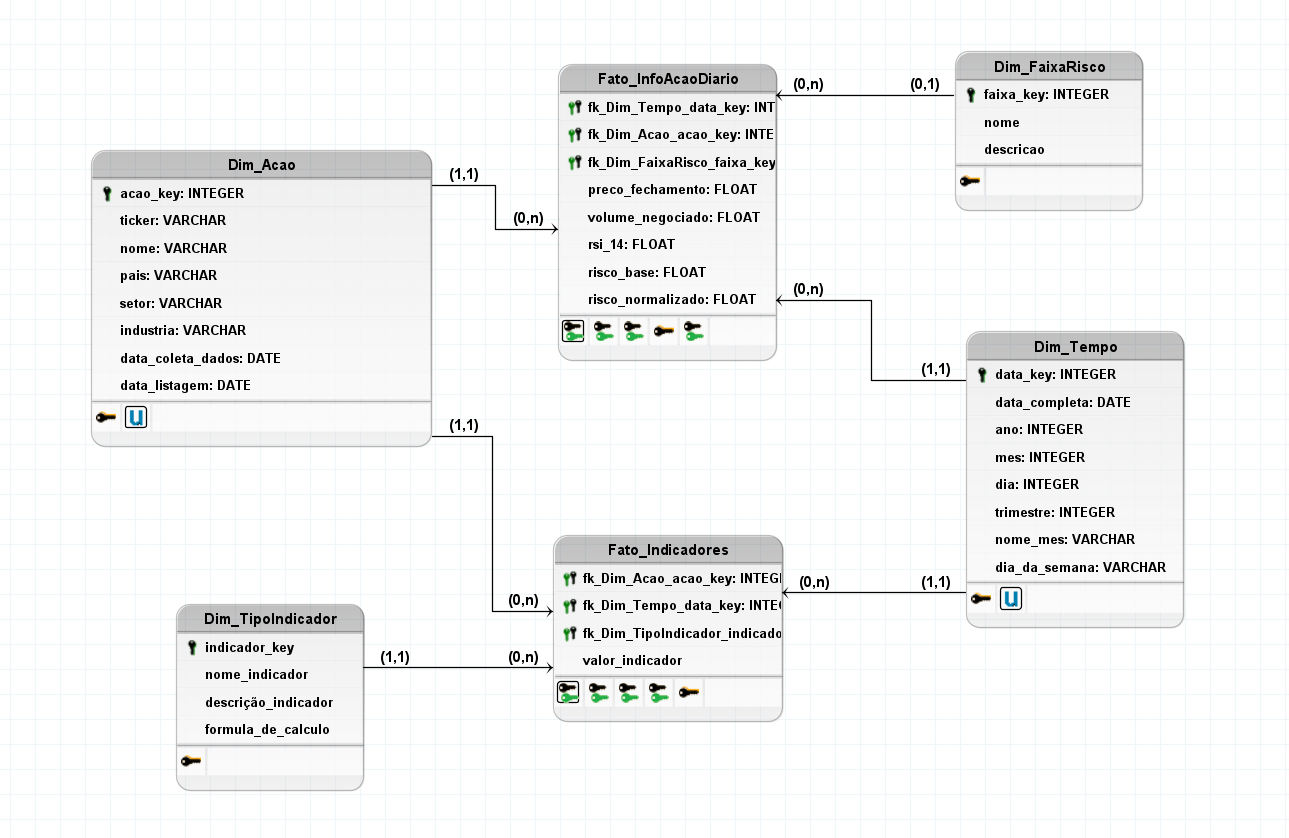
\includegraphics[width=0.9\textwidth]{figuras/logico_2.png}
\fonte{Elaborada pelo autor.}
\end{figure}

\section{Planejamento do ETL}
\label{sec:planejamento-etl}

Definido o modelo dimensional, é necessário planejar o processo de Extração, Transformação e Carga (ETL) que povoará esse repositório a partir dos artefatos brutos produzidos pela coleta descrita na Seção \ref{coleta}. Esse planejamento precede qualquer decisão de ferramenta ou implementação, e foi conduzido em três etapas.

A primeira etapa consistiu na identificação dos artefatos brutos produzidos pelos scripts de coleta, delimitando os arquivos de entrada. A segunda etapa estabeleceu o mapeamento entre os campos desses artefatos e os atributos das tabelas do modelo dimensional apresentado na Seção~\ref{sec:modelagem-dimensional}, incluindo o tratamento requerido em cada correspondência (renomeação, conversão de tipo, cálculo derivado ou agregação). A terceira etapa organizou essas correspondências em uma sequência lógica de transformações, cujo resultado orienta a implementação do fluxo apresentada na Seção \ref{sec:pipeline-etl}.

O mapeamento de-para consolidado durante a segunda etapa do planejamento é apresentado na Tabela~\ref{tab:mapeamento-etl}. Ele documenta a origem de cada atributo materializado no \textit{data mart}, a transformação aplicada até a carga e a tabela de destino, permitindo a rastreabilidade completa entre o dado bruto e o dado consumido pelas consultas analíticas.

{\footnotesize
\begin{longtable}{|p{4cm}|p{5cm}|p{2cm}|p{3cm}|}
\caption{Mapeamento de-para entre os campos do dado bruto e os atributos do modelo dimensional.}
\label{tab:mapeamento-etl}\\
\hline
\textbf{Campo Origem} & \textbf{Transformação} & \textbf{Tabela Destino} & \textbf{Campo Destino} \\ \hline
\endfirsthead

\multicolumn{4}{c}{\tablename\ \thetable\ -- Continuação}\\
\hline
\textbf{Campo Origem (JSON Path)} & \textbf{Transformação} & \textbf{Tabela Destino} & \textbf{Campo Destino} \\ \hline
\endhead

\hline
\multicolumn{4}{r}{\textit{Continua na próxima página}}\\
\endfoot

\hline
\endlastfoot

N/A & Gerado automaticamente (PK) & \texttt{Dim\_Acao} & \texttt{acao\_key} \\ \hline
Chave raiz do objeto JSON (ex.: ``AAL'') & Nenhuma & \texttt{Dim\_Acao} & \texttt{ticker} \\ \hline
\texttt{info\_gerais.nome} & Nenhuma & \texttt{Dim\_Acao} & \texttt{nome} \\ \hline
\texttt{info\_gerais.country} & Nenhuma & \texttt{Dim\_Acao} & \texttt{pais} \\ \hline
\texttt{info\_gerais.setor} & Nenhuma & \texttt{Dim\_Acao} & \texttt{setor} \\ \hline
\texttt{info\_gerais.industria} & Nenhuma & \texttt{Dim\_Acao} & \texttt{industria} \\ \hline
\ttbreak{info\_gerais.\_valor\_mercado\_atual} & Manter tipo numérico (FLOAT/REAL) & \texttt{Dim\_Acao} & \ttbreak{ultimo\_valor\_mercado\_disponivel} \\ \hline
\texttt{info\_gerais.pl\_atual} & Se NaN, converter para ``não informado'' & \texttt{Dim\_Acao} & \ttbreak{ultimo\_pl\_disponivel} \\ \hline
\texttt{info\_gerais.pvpa\_atual} & Manter tipo numérico; aceitar NULL/NaN & \texttt{Dim\_Acao} & \ttbreak{ultimo\_pvpa\_disponivel} \\ \hline
\ttbreak{info\_gerais.trailing\_dividend\_yield} & Manter tipo numérico; aceitar NULL/NaN & \texttt{Dim\_Acao} & \ttbreak{ultimo\_yield\_dividendo\_disponivel} \\ \hline
\ttbreak{info\_gerais.five\_year\_avg\_dividend\_yield} & Manter tipo numérico; aceitar NULL/NaN & \texttt{Dim\_Acao} & \ttbreak{ultimo\_yield\_dividendo\_5a\_disponivel} \\ \hline
\ttbreak{info\_gerais.ebitda\_margin} & Manter tipo numérico; aceitar NULL/NaN & \texttt{Dim\_Acao} & \ttbreak{ultimo\_margem\_ebitda\_disponivel} \\ \hline
\ttbreak{info\_gerais.enterprise\_to\_ebitda} & Manter tipo numérico; aceitar NULL/NaN & \texttt{Dim\_Acao} & \ttbreak{ultimo\_ev\_ebitda\_disponivel} \\ \hline
\ttbreak{info\_gerais.price\_to\_sales} & Manter tipo numérico; aceitar NULL/NaN & \texttt{Dim\_Acao} & \ttbreak{ultimo\_price\_to\_sales\_disponivel} \\ \hline
\ttbreak{info\_gerais.data\_listagem} & Nenhuma & \texttt{Dim\_Acao} & \texttt{data\_coleta\_dados} \\ \hline
\ttbreak{info\_gerais.data\_de\_coleta} & Nenhuma & \texttt{Dim\_Acao} & \texttt{data\_listagem} \\ \hline
\ttbreak{dados\_historicos[].data} & Remover hífens para criar inteiro (ex.: ``2021-03-24'' $\rightarrow$ 20210324) & \texttt{Dim\_Tempo} & \texttt{data\_key} (PK) \\ \hline
\ttbreak{dados\_historicos[].data} & Manter formato \textit{string} original ``YYYY-MM-DD'' & \texttt{Dim\_Tempo} & \texttt{data\_completa} \\ \hline
\ttbreak{dados\_historicos[].data} & Extrair apenas a parte do ano (YYYY) & \texttt{Dim\_Tempo} & \texttt{ano} \\ \hline
\ttbreak{dados\_historicos[].data} & Extrair apenas a parte do mês (MM) & \texttt{Dim\_Tempo} & \texttt{mes} \\ \hline
\ttbreak{dados\_historicos[].data} & Extrair apenas a parte do dia (DD) & \texttt{Dim\_Tempo} & \texttt{dia} \\ \hline
\ttbreak{dados\_historicos[].data} & Calcular trimestre baseado no mês $((\text{mês}-1)//3 + 1)$ & \texttt{Dim\_Tempo} & \texttt{trimestre} \\ \hline
\ttbreak{dados\_historicos[].data} & Derivar nome do mês (ex.: ``Janeiro'') & \texttt{Dim\_Tempo} & \texttt{nome\_mes} \\ \hline
\ttbreak{dados\_historicos[].data} & Derivar dia da semana & \texttt{Dim\_Tempo} & \texttt{dia\_da\_semana} \\ \hline
Derivado do ETL (Indicador) & \textit{Lookup} na \ttbreak{Dim\_TipoIndicador} & \ttbreak{Fato\_Indicadores} & \texttt{indicador\_key} (FK) \\ \hline
Nome do índice (ex.: ``S\&P\_Low\_PL'') & Nenhuma & \ttbreak{Dim\_TipoIndicador} & \texttt{nome\_indicador} \\ \hline
Descrição do perfil do índice & Nenhuma & \ttbreak{Dim\_TipoIndicador} & \ttbreak{descricao\_indicador} \\ \hline
Definição matemática do indicador & Nenhuma & \ttbreak{Dim\_TipoIndicador} & \ttbreak{formula\_de\_calculo} \\ \hline
Derivado do ETL (Ticker) & \textit{Lookup} na dimensão: buscar \texttt{acao\_key} na \texttt{Dim\_Acao} & \ttbreak{Fato\_InfoAcao} & \texttt{acao\_key} (FK) \\ \hline
Derivado do ETL (Data) & \textit{Lookup} na dimensão: buscar \texttt{data\_key} na \texttt{Dim\_Tempo} & \ttbreak{Fato\_InfoAcao} & \texttt{data\_key} (FK) \\ \hline
\ttbreak{dados\_historicos[].preco\_fechamento} & Manter tipo numérico (FLOAT/REAL) & \ttbreak{Fato\_InfoAcao} & \texttt{preco\_fechamento} \\ \hline
\ttbreak{dados\_historicos[].volume} & Manter tipo numérico (FLOAT/REAL) & \ttbreak{Fato\_InfoAcao} & \texttt{volume} \\ \hline
\ttbreak{dados\_historicos[].rsi\_14} & Manter tipo numérico; converter ``NaN'' para NULL & \ttbreak{Fato\_InfoAcao} & \texttt{rsi\_14} \\ \hline
Derivado do ETL (Ticker) & \textit{Lookup} na \texttt{Dim\_Acao} & \ttbreak{Fato\_Indicadores} & \texttt{acao\_key} (FK) \\ \hline
Derivado do ETL (Data) & \textit{Lookup} na \texttt{Dim\_Tempo} & \ttbreak{Fato\_Indicadores} & \texttt{data\_key} (FK) \\ \hline
Derivado do ETL (Indicador) & \textit{Lookup} na \ttbreak{Dim\_TipoIndicador} & \ttbreak{Fato\_Indicadores} & \texttt{indicador\_key} (FK) \\ \hline
Resultado do cálculo & Valor numérico final do índice & \ttbreak{Fato\_Indicadores} & \texttt{valor\_indicador} \\ \hline

\end{longtable}
}

\fonte{Elaborado pelos autores.}

\section{Implementação do \textit{Pipeline} ETL}
\label{sec:pipeline-etl}

A partir do planejamento apresentado na Seção \ref{sec:planejamento-etl}, o \textit{pipeline} foi orquestrado no Tableau Prep Builder, uma ferramenta visual de preparação de dados, cujos nós encapsulam as transformações identificadas na fase de planejamento e as aplicam sobre os arquivos brutos coletados pelos scripts em Python. A Figura~\ref{fig:fluxo-etl} apresenta o fluxo em alto nível, com os passos renomeados para descrições funcionais que tornam imediata a leitura da jornada do dado, do artefato bruto ao carregamento nas tabelas fato e nas tabelas dimensão.

\begin{figure}[ht]
\centering
\caption{Fluxo ETL em alto nível}
\label{fig:fluxo-etl}
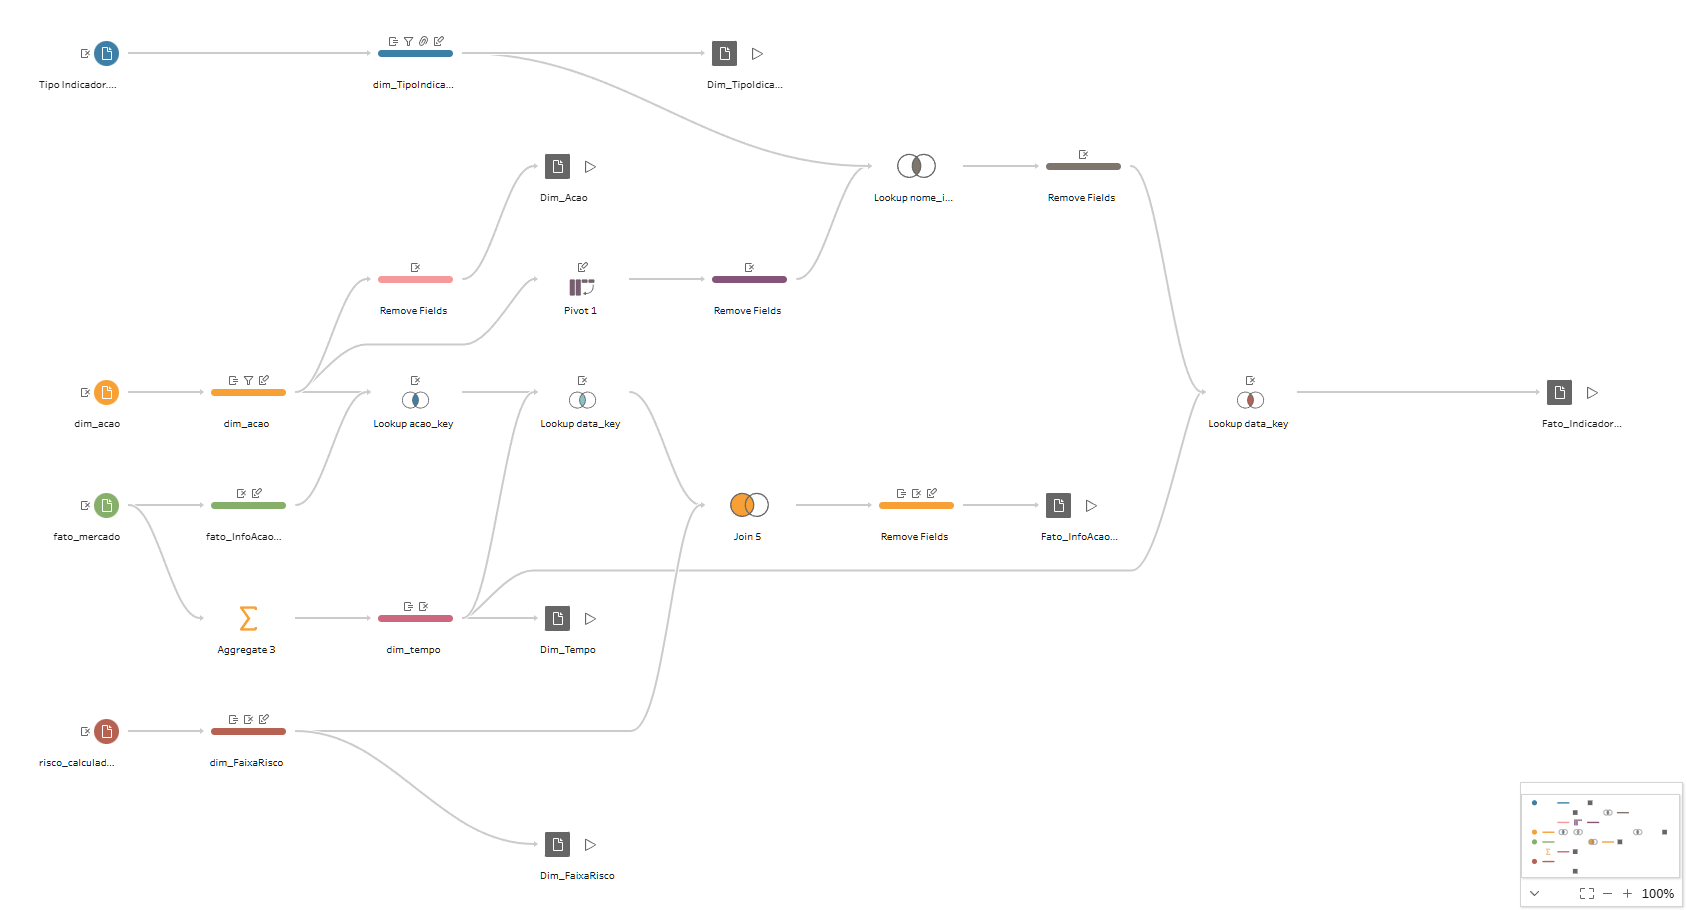
\includegraphics[width=\textwidth]{figuras/fluxo2.png}
\fonte{Elaborada pelo autor.}
\end{figure}

A jornada começa nos arquivos JSON gerados pela camada de coleta, que consolidam, por \textit{ticker}, o histórico de preços a partir de 2010, o conjunto de fundamentos corporativos no instante da extração e os metadados descritivos da empresa, como setor, indústria e país. Esses arquivos são lidos como entradas no fluxo de ETL e, em seguida, sofrem uma desnormalização controlada que separa os atributos descritivos, candidatos à dimensão de ação, dos atributos mensuráveis, candidatos às tabelas fato.

A etapa seguinte aplica as regras de tratamento descritas na Seção~\ref{sec:tratamento-dados}, incluindo a exclusão por reaproveitamento de \textit{ticker}, a remoção de ativos com janela histórica insuficiente e a filtragem de \textit{outliers} cuja amplitude comprometeria a legibilidade gráfica. A dimensão de tempo é gerada de forma sintética, varrendo o intervalo coberto pelas séries e materializando os atributos derivados de cada data. Os indicadores são pivotados do formato horizontal de coleta para o formato verticalizado da tabela \texttt{Fato\_Indicadores}, com a inclusão da chave estrangeira que aponta para a dimensão de tipo de indicador.

O mapeamento de campos entre as saídas do fluxo visual e o esquema do banco precisou conciliar dois vocabulários distintos. As chaves \texttt{data\_key} e \texttt{acao\_key} dos arquivos intermediários são renomeadas para \texttt{fk\_dim\_tempo\_data\_key} e \texttt{fk\_dim\_acao\_acao\_key} no momento da carga, respeitando a convenção de nomenclatura adotada no \textit{data mart}. De forma análoga, a coluna \texttt{data\_de\_coleta} é renomeada para \texttt{data\_coleta\_dados} na dimensão de ação, e a coluna \texttt{data} é renomeada para \texttt{data\_completa} na dimensão de tempo. Esse remapeamento é aplicado em tempo de carga por um \textit{script} de orquestração, que segue um plano sequencial garantindo que as dimensões sejam carregadas antes dos fatos, em conformidade com as restrições de integridade referencial.

\section{Tratamento de Dados}
\label{sec:tratamento-dados}

A etapa de tratamento é aplicada durante o \textit{pipeline} ETL descrito na Seção \ref{sec:pipeline-etl}, entre a leitura dos artefatos brutos e a carga nas tabelas fato e dimensão descritas na Seção \ref{sec:modelagem-dimensional}. Seu propósito é converter o conjunto bruto de dados em uma base coerente, livre de registros inválidos e estatisticamente adequada ao cálculo das métricas de risco descritas no capítulo de fundamentação. Em conformidade com a recomendação de \citeonline{barbieri_bi_2001}, as exclusões de registros e os cálculos derivados foram concentrados nesta parte da modelagem, de modo que o repositório analítico final entregue ao usuário apresente os dados já saneados e prontos para consulta, sem necessidade de filtragens reativas na camada de visualização.

\subsection{Limpeza e Padronização}

A primeira iteração do tratamento concentra-se na higienização dos atributos coletados. Ela contempla a uniformização de tipos de dados, a conversão de campos textuais em representações numéricas quando aplicável, a normalização de identificadores de ativos (\textit{tickers}) e a verificação de integridade referencial entre as séries históricas de preço e os atributos descritivos de cada empresa. Registros com identificador ausente, com data inválida ou cujo provedor público de dados financeiros não retornou informação de fechamento foram descartados, uma vez que comprometem a continuidade da série temporal exigida pelos cálculos subsequentes.

Atributos ausentes receberam tratamento distinto dos atributos de preço. Como esses indicadores são valores pontuais associados ao momento da coleta, a ausência de um campo específico não invalida o ativo como um todo, e a ausência foi preservada como informação semântica, permitindo que o modelo de risco aplique apenas os modificadores efetivamente disponíveis para cada empresa.

\subsection{Tratamento de Carência Estatística}

As métricas que sustentam o \textit{score} de risco proposto, em particular a volatilidade amostral e o coeficiente Beta, exigem uma janela móvel mínima de observações para que sua estimativa apresente significância estatística. Em decorrência dessa exigência, os primeiros dias da série histórica de cada ativo não dispõem de massa suficiente para alimentar o cálculo, gerando o que se denomina, no contexto deste trabalho, carência estatística. O tratamento adotado consiste em registrar nulidade explícita para o \textit{score} de risco nesses intervalos iniciais, em vez de imputar valores estimados ou propagar a primeira observação válida.

A opção pela nulidade explícita se justifica, já que qualquer imputação introduziria sinal artificial em uma região na qual a métrica é, por construção, indeterminada. Além disso, permite que as consultas analíticas subsequentes filtrem de maneira transparente os períodos em que o ativo ainda não dispõe de risco calculado, preservando a auditabilidade do \textit{pipeline}. A extensão da carência é determinada pelo tamanho da janela de cálculo adotada para a volatilidade e o Beta, e os ativos cuja série histórica disponível é menor do que essa janela mínima são automaticamente excluídos do escopo analítico.

\subsection{Remoção de \textit{Outliers}}

A última etapa do tratamento consiste em remover ativos cujos retornos ou indicadores apresentam valores extremos, suficientemente distantes do restante do universo para distorcer as análises. Esses ativos comprometem o estudo tanto na visualização, tendo em vista que poucos pontos extremos passam a definir a escala dos gráficos comparativos de retorno, comprimindo os demais ativos em uma faixa visualmente indistinta. Quanto na padronização via \textit{Z-score} aplicada aos modificadores, valores extremos inflam o desvio padrão populacional e reduzem artificialmente as distâncias relativas entre os ativos típicos.

A esse critério estatístico soma-se um critério de integridade referencial. Identificou-se um ativo cujo \textit{ticker} foi reaproveitado ao longo do período analisado para representar empresas distintas, em decorrência de descontinuidade da empresa original e posterior alocação do mesmo código a uma nova listagem. Como a série histórica associada a esse \textit{ticker} não corresponde a uma entidade econômica única, sua manutenção comprometeria tanto o cálculo das métricas de risco, que pressupõem continuidade do ativo subjacente, quanto a interpretação dos resultados agregados. O ativo foi, portanto, excluído do universo de análise.

A remoção, em ambos os critérios, é executada na camada de transformação do \textit{ETL} e gravada no repositório analítico final, e não aplicada como filtro pontual em cada consulta. Centralizar a regra no \textit{ETL} garante que todas as visualizações operem sobre o mesmo universo e documenta de forma explícita o conjunto efetivo de ativos avaliados. Os ativos removidos são tratados como exclusão deliberada, justificada pelo seu impacto estatístico ou pela quebra de integridade referencial da série histórica, e não como perda de informação.

\section{Modelagem do Grau de Risco}
\label{sec:modelagem-risco}

Concluído o tratamento descrito na seção anterior, a etapa seguinte da metodologia consiste em transformar o conjunto saneado de séries históricas e atributos descritivos em uma métrica única, capaz de ordenar os ativos segundo seu nível de risco. A modelagem proposta é construída em quatro estágios sequenciais. Primeiro, calculam-se duas métricas de risco com fundamentação teórica consolidada, conforme apresentado no capítulo \ref{fundamentacao}. Em seguida, essas duas métricas são unificadas em um único \textit{score} via padronização estatística. O \textit{score} resultante é então remapeado para uma escala fechada de interpretação intuitiva. Por fim, define-se uma classificação categórica derivada desse \textit{score}, materializada diretamente no repositório analítico.

\subsection{Volatilidade Anualizada}

A primeira dimensão do risco capturada pelo modelo é a volatilidade do próprio ativo, entendida como medida de dispersão dos seus retornos diários em torno da média. O cálculo aplica o desvio padrão amostral sobre uma janela móvel de retornos logarítmicos, conforme apresentado na equação \ref{eq:volatilidade-amostral} \cite{assaf_neto_mercado_2022}, e em seguida é anualizado pela multiplicação por \(\sqrt{n}\), em que \(n\) é o número de períodos de negociação contidos em um ano. A anualização garante que a métrica seja diretamente comparável a \textit{benchmarks} de mercado e a estudos da literatura, que tradicionalmente reportam volatilidade em base anual.

\begin{equation}
\label{eq:volatilidade-amostral}
s = \sqrt{\frac{\sum_{i=1}^{n} (R_i - \bar{R})^2}{n - 1}}
\end{equation}

\noindent em que \(R_i\) representa o retorno do ativo na data \(i\), \(\bar{R}\) a média dos retornos no intervalo da janela e \(n\) o tamanho dessa janela. A volatilidade assim definida captura o que a literatura denomina risco idiossincrático, isto é, a parcela do risco específica ao comportamento do próprio ativo, independentemente do contexto de mercado.

\subsection{Coeficiente Beta com Referência ao S\&P 500}

A segunda dimensão do risco refere-se à sensibilidade do ativo em relação ao movimento agregado do mercado, capturada pelo coeficiente Beta. Esse coeficiente é estimado por meio da razão entre a covariância dos retornos do ativo com os retornos do índice de referência e a variância dos retornos desse mesmo índice, conforme expresso na equação \ref{eq:beta} \cite{sharpe1964}.

\begin{equation}
\label{eq:beta}
\beta = \frac{\sum_{i=1}^{n} (R_{a,i} - \bar{R}_a)(R_{m,i} - \bar{R}_m)}{\sum_{i=1}^{n} (R_{m,i} - \bar{R}_m)^2}
\end{equation}

\noindent em que \(R_{a,i}\) é o retorno do ativo na data \(i\), \(R_{m,i}\) o retorno do índice de referência na mesma data, e \(\bar{R}_a\) e \(\bar{R}_m\) as respectivas médias no intervalo da janela. O índice S\&P 500 foi adotado como \textit{benchmark} único de mercado, decisão justificada por sua aceitação consolidada como representação do mercado acionário norte-americano e pelo alinhamento com o escopo geográfico do estudo, restrito a ativos negociados nas bolsas NYSE e NASDAQ. Diferentemente da volatilidade, o Beta captura o risco sistêmico, ou seja, a parcela do risco que decorre da exposição do ativo aos movimentos comuns ao mercado como um todo.

\subsection{Unificação por \textit{Z-score}}

Volatilidade anualizada e coeficiente Beta possuem naturezas matemáticas distintas, expressas em escalas e ordens de grandeza incompatíveis entre si. A primeira é uma medida estritamente positiva apresentada em escala percentual, enquanto o segundo é um número real centrado em torno da unidade e que pode assumir valores negativos para ativos com correlação inversa ao mercado. Combiná-las diretamente, por soma ou média aritmética, distorceria a composição final em favor da métrica com maior amplitude absoluta.

Para contornar essa incompatibilidade, ambas as métricas são submetidas a padronização estatística pelo \textit{Z-score}, conforme a equação \ref{eq:z-score}, calculado sobre a população de ativos observada no mesmo recorte temporal de referência.

\begin{equation}
\label{eq:z-score}
Z = \frac{x - \mu}{\sigma}
\end{equation}

\noindent em que \(x\) é o valor original da métrica para o ativo avaliado, \(\mu\) a média da métrica no universo de ativos no recorte temporal considerado e \(\sigma\) o desvio padrão correspondente. Após a padronização, ambas as métricas passam a estar centradas em zero e dimensionadas em unidades de desvio padrão, tornando-se aritmeticamente comparáveis. O \textit{score} de risco base é então definido como a média aritmética dos dois \textit{Z-scores}, conforme expresso na equação \ref{eq:risco-base}.

\begin{equation}
\label{eq:risco-base}
\text{risco}_{\text{base}} = \frac{Z_{s} + Z_{\beta}}{2}
\end{equation}

A escolha por pesos iguais entre as duas dimensões reflete a decisão metodológica de não privilegiar a priori nem o risco idiossincrático nem o risco sistêmico, deixando essa eventual ponderação como possível extensão do modelo. O \textit{score} resultante posiciona cada ativo em relação ao comportamento típico do universo analisado, com valores positivos indicando risco superior à média e valores negativos indicando risco inferior.

\subsection{Normalização Min-Max}

O \textit{score} de risco base, expresso em unidades de desvio padrão, é estatisticamente coerente, porém pouco intuitivo para fins de visualização e interpretação por usuários finais. Para mitigar essa limitação, aplica-se uma normalização Min-Max sobre o conjunto histórico agregado de \textit{score}s, remapeando-os para o intervalo fechado de 0 a 100, conforme a equação \ref{eq:min-max}.

\begin{equation}
\label{eq:min-max}
\text{risco}_{\text{normalizado}} = \left( \frac{R_i - R_{\min}}{R_{\max} - R_{\min}} \right) \times 100
\end{equation}

\noindent em que \(R_i\) é o \textit{score} de risco base do registro avaliado, e \(R_{\min}\) e \(R_{\max}\) os limites mínimo e máximo observados na população histórica completa. A normalização preserva integralmente a ordenação relativa entre os ativos e, ao produzir um indicador na escala de 0 a 100, viabiliza sua incorporação direta em interfaces analíticas e em comparações intuitivas entre ativos, sem alterar a substância estatística do \textit{score} original.

\subsection{Faixas de Risco}
\label{subsec:faixas-risco}

A última etapa da modelagem traduz o \textit{score} contínuo em uma classificação categórica composta por cinco faixas, denominadas Muito Baixo, Baixo, Médio, Alto e Muito Alto. A motivação para essa categorização é dupla. Sob o ponto de vista analítico, a discretização viabiliza agrupamentos diretos para comparações entre coortes de ativos, como cálculo de retorno médio por faixa, exposição setorial e análise de \textit{drawdown}. Sob o ponto de vista comunicacional, ela aproxima o modelo da linguagem usual da indústria de investimentos, em que perfis de risco são tipicamente expressos em rótulos qualitativos.

A calibração das fronteiras entre as faixas foi conduzida a partir do exame da distribuição empírica do \textit{score} de risco base sobre toda a massa de dados disponível. Foram avaliadas três estratégias alternativas. A primeira consistiu na aplicação de cortes fixos tradicionais, baseados em múltiplos inteiros do desvio padrão. A segunda dividiu o intervalo total em cinco partes de amplitude uniforme. A terceira utilizou cortes derivados de quantis da distribuição observada, particionando a população em cinco subconjuntos de tamanho equivalente.

As duas primeiras estratégias produziram distribuições insatisfatórias para os propósitos do estudo, concentrando a maioria expressiva dos registros em uma única faixa central e esvaziando as faixas extremas. Esse comportamento decorre da assimetria e da presença de caudas longas na distribuição observada, característica recorrente em séries financeiras. A estratégia baseada em quantis, por outro lado, produziu uma distribuição equitativa em volume e revelou as fronteiras empíricas naturais entre os comportamentos de risco no universo analisado.

A partir dessa observação, optou-se por uma calibração híbrida, em que as fronteiras entre as faixas são derivadas dos limites dos quantis observados, porém arredondadas e espelhadas em torno do zero, de modo a produzir uma estrutura simétrica em relação ao \textit{score} neutro de mercado. A simetria confere ao modelo o benefício da classificação interpretável de forma direta, já que cada faixa positiva tem uma contraparte negativa de mesma amplitude. As fronteiras adotadas são apresentadas na Tabela \ref{tab:faixas-risco}.

\begin{table}[htb]
\centering
\caption{Definição das faixas de risco}
\label{tab:faixas-risco}
\renewcommand{\arraystretch}{1.6}
\begin{supertabular}{m{4.0cm}m{7.0cm}}
\hline
\multicolumn{1}{m{4.0cm}|}{\centering \textbf{Faixa}} &
\centering\arraybslash \textbf{Condição sobre o risco base}\\\hline
\centering Muito Baixo &
\centering\arraybslash \(\text{risco}_{\text{base}} \leq -0{,}60\)\\
\centering Baixo &
\centering\arraybslash \(-0{,}60 < \text{risco}_{\text{base}} \leq -0{,}25\)\\
\centering Médio &
\centering\arraybslash \(-0{,}25 < \text{risco}_{\text{base}} \leq 0{,}25\)\\
\centering Alto &
\centering\arraybslash \(0{,}25 < \text{risco}_{\text{base}} \leq 0{,}60\)\\
\centering Muito Alto &
\centering\arraybslash \(\text{risco}_{\text{base}} > 0{,}60\)\\\hline
\end{supertabular}
\end{table}

A faixa central, denominada Médio, opera como uma zona neutra, agrupando ativos cujo \textit{score} não se distancia significativamente do comportamento típico do universo. As demais faixas representam afastamentos progressivos dessa neutralidade em direção a perfis de menor ou maior risco.

A estrutura simétrica de cinco faixas também dialoga com a categorização de perfis de investidor discutida na Seção~\ref{perfil investidor}. \citeonline{assaf_neto_mercado_2022} que organiza o investidor em três perfis clássicos, conservador, moderado e arrojado, definidos por limiares percentuais de perda tolerada. A correspondência com as faixas propostas neste trabalho não é matemática, uma vez que os cortes de \citeonline{assaf_neto_mercado_2022} operam sobre uma escala absoluta de perda enquanto as faixas derivam da posição relativa do ativo na distribuição do universo, mas é interpretativa: as faixas Muito Baixo e Baixo agrupam ativos compatíveis com o perfil conservador, a faixa Médio corresponde ao perfil moderado, e as faixas Alto e Muito Alto ao perfil arrojado. A adoção de cinco faixas em vez de três é o que viabiliza o desdobramento em perfis intermediários, no qual um investidor conservador com maior tolerância pode transitar para o extremo superior da faixa Baixo, e um investidor arrojado com aversão a perdas extremas pode se acomodar no extremo inferior da faixa Alto, sem que essa especificidade extra exija duplicação da estrutura de dados nem alteração da fórmula de risco.

\subsection{Materialização das Faixas no Repositório Analítico}

A classificação categórica descrita acima foi incorporada ao repositório analítico como dimensão própria, referenciada por chave estrangeira a partir da tabela fato de informações diárias, conforme já apresentado na Seção \ref{sec:modelagem-dimensional}. Desta forma, a definição das faixas constitui regra de negócio do modelo, e não preferência transitória de visualização. Mantê-la em camada de transformação garante que toda consulta executada sobre o repositório, independentemente da ferramenta de visualização que a invoque, observe a mesma classificação. Distribuir essa regra entre múltiplas consultas exporia o modelo ao risco de divergências silenciosas, em que pequenas variações na expressão lógica produziriam recortes diferentes para o mesmo conjunto de dados.

Outro ponto positivo é o impacto no desempenho. Cláusulas condicionais aplicadas em tempo de consulta sobre conjuntos volumétricos exigem reavaliação a cada execução, ao passo que um atributo previamente calculado e indexado permite agregações e filtragens diretas, com custo computacional substancialmente inferior. E ao materializar a faixa como dimensão documentada de forma explícita, no próprio repositório, o resultado da regra de classificação, o modelo se torna inspecionável sem necessidade de reconstruir mentalmente a lógica de cada consulta.

\section{Lógica de Alocação da Carteira}
\label{sec:alocacao-carteira}

A construção da carteira de investimento neste trabalho abandona os critérios discricionários comuns ao investidor individual, como recomendações de analistas, preferências subjetivas ou tentativas iterativas de calibração manual, e adota um procedimento determinístico que pode ser auditado, reproduzido e contestado. A lógica se apoia em uma função de ordenação que converte os indicadores econômicos da empresa, padronizados em relação ao universo analisado, em peso percentual via transformação exponencial natural, e uma estratificação categórica do risco que torna a inclusão de cada ativo na carteira justificável.

\subsection{Ordenação por Score de Qualidade e Transformação Exponencial}
Cada ação $i$ recebe um Score de Qualidade composto pela média ponderada dos \textit{Z-scores} dos três modificadores e da penalidade pelo seu risco médio histórico:

\begin{equation}
\label{eq:score-qualidade}
\text{Score}_i \;=\; \frac{
  -\,\alpha_{DY}\, Z_{DY,i}
  \;+\; \alpha_{EB}\, Z_{EB,i}
  \;-\; \alpha_{EV}\, Z_{EV,i}
  \;-\; \overline{R_i}
}{
  \alpha_{DY} + \alpha_{EB} + \alpha_{EV} + 1
}
\end{equation}

em que $Z_{x,i} = (x_i - \mu_x)/\sigma_x$ é o desvio padronizado da ação em relação à média do universo amostrado; $\overline{R_i}$ é o risco normalizado médio do ativo no período; e $\alpha_x \in \{0, 1\}$ são interruptores que permitem incluir ou excluir cada fator analiticamente. O sinal de cada termo reflete a interpretação econômica do indicador: a margem EBITDA atua como amortecedor, subtraindo do risco, enquanto $EV/EBITDA$ elevado e \textit{Trailing Dividend Yield} elevado atuam como amplificadores.

O \textit{Score} em si, contudo, é insuficiente para gerar um peso de alocação: ele assume valores positivos e negativos, com magnitudes muito próximas entre ativos rivais, e somá-los diretamente não produziria uma distribuição percentual válida. A solução adotada submete o score a uma transformação exponencial baseada no número de Euler ($e \approx 2{,}71828$):

\begin{equation}
\label{eq:peso-bruto}
w_i^{\text{bruto}} \;=\; e^{\,\max(-5,\ \min(5,\ \text{Score}_i))}
\end{equation}

A alocação final dentro de cada setor $s$ é obtida pela normalização desses pesos brutos:

\begin{equation}
\label{eq:peso-final}
w_i^{\text{final}} \;=\; \frac{w_i^{\text{bruto}}}{\displaystyle\sum_{j \in s} w_j^{\text{bruto}}} \times 100
\end{equation}

Esta construção é matematicamente equivalente a uma função \textit{softmax} sem parâmetro de temperatura, amplamente empregada em aprendizado de máquina e em modelos de escolha discreta em econometria, notavelmente no \textit{logit} multinomial de \citeonline{mcfadden1973}. A escolha do número de Euler como base da exponencial não é arbitrária: $e$ é a única base para a qual $\frac{d}{dx}e^x = e^x$, propriedade que garante que a função preserva sua estrutura sob derivação e integração, característica fundamental quando se deseja que pequenas variações no Score se traduzam em variações suaves no peso final.

O recorte do Score no intervalo $[-5,\, +5]$ antes da exponenciação evita problemas numéricos: valores fora desse intervalo gerariam pesos da ordem de $e^{\pm 5} \approx 148{,}4$ ou $\approx 0{,}0067$, suficientes para distinguir extremos sem causar \textit{overflow} ou \textit{underflow} nos cálculos subsequentes.

\subsection{Faixas de Risco como Critério Objetivo de Inclusão}
\label{subsec:faixas-inclusao}

Uma fragilidade clássica das estratégias quantitativas implementadas por investidores individuais é a seleção de ativos por tentativa e erro. Carteiras montadas dessa forma sofrem de duas limitações simultâneas, a impossibilidade de justificar formalmente a inclusão de cada ativo e a vulnerabilidade a vieses cognitivos como familiaridade, ancoragem e excesso de confiança documentados por \citeonline{kahneman_prospect_1979}.

Este trabalho propõe substituir esse processo discricionário pelo conceito de faixa de risco, atributo categórico atribuído a cada ação a partir da quantilização do risco normalizado em cinco intervalos: ``1 -- Muito Baixo'', ``2 -- Baixo'', ``3 -- Médio'', ``4 -- Alto'' e ``5 -- Muito Alto''. Esses intervalos derivam diretamente da composição estatística de volatilidade anualizada ($\sigma$) e Beta ($\beta$) descrita na Seção~\ref{sec:modelagem-risco}, e portanto carregam significado quantitativo bem definido em vez de classificação narrativa.

Esta metodologia produz uma carteira cuja construção pode ser descrita em termos formais auditáveis: admitem-se apenas ativos pertencentes a um conjunto $\mathcal{F}$ de faixas de risco previamente escolhido pelo investidor; atribui-se a cada ativo admissível um Score de Qualidade \textit{Z}-padronizado contra a média do universo, conforme a Equação~\ref{eq:score-qualidade}; e a alocação percentual final é obtida pela normalização \textit{softmax} dos scores dentro de cada setor, conforme as Equações~\ref{eq:peso-bruto} e~\ref{eq:peso-final}.

